\documentclass[12pt]{article}
\usepackage{latexsym}
\usepackage{amssymb,amsmath}
\usepackage{float}
\usepackage{graphicx}
\textwidth=6in \textheight=8.5in

\restylefloat{figure}

\begin{document}\begin{center}
CS 181\\
Problem Set 1\\
Ina Chen and Kathy Lin
\end{center}

\begin{enumerate}

	\item 
		\begin{enumerate}
			\item Here is the breakdown of the data:\\\\
				\begin{tabular}{|c|c|c|}
        				\hline
        				~            & 1 & 0 \\ \hline
        				A = 1 & 2      & 2      \\ 
        				A = 0 & 2      & 1      \\
        				\hline
        				B = 1 & 1      & 1      \\ 
        				B = 0 & 3      & 2      \\
        				\hline
					Total & 4      & 3      \\
        				\hline
    				\end{tabular}
\\\\\\Let $Y$ represent the space of the label
				\begin{align*}Information gain &= H(Y) - H(Y|X)\\
							& = H(Y) -\Sigma_{x,y}p(x|y)log_{2}\frac{1}{p(x|y)}\end{align*}
				$H(Y) = \frac{4}{7}log_{2}\frac{7}{4} + \frac{3}{7}log_{2}\frac{7}{3} = 0.985$\\\\
				For A:\\\\
				$H(Y|A = 1) = 0.5log_{2}2 + 0.5log_{2}2 = 1$\\
				$H(Y|A = 0) = \frac{2}{3}log_{2}\frac{3}{2} + \frac{1}{3}log_{2}3 = 0.918$\\
				$H(Y|A) = \frac{4}{7}(1) + \frac{3}{7}0.918 = 0.965$\\
				$I(A ; Y) = 0.985 - 0.965 = \fbox{0.02}$\\

				For B:\\\\
				$H(Y|B = 1) = 0.5log_{2}2 + 0.5log_{2}2 = 1$\\
				$H(Y|B = 0) = \frac{2}{5}log_{2}\frac{5}{3} + \frac{2}{5}log_{2}\frac{5}{2} = 0.971$\\
				$H(Y|B) = \frac{4}{7}(1) + \frac{3}{7}(0.971) = 0.979$\\
				$I(B ; Y) = 0.985 - 0.979 = \fbox{0.006}$\\

				Since A has more mutual information with the label, ID3 would split on attribute A. Splitting on A could be more useful because even though A = 1 does not give any extra information, when A = 0, the distribution becomes split into 1/3 and 2/3. This is better than when B = 0, when the distribution becomes 2/5 and 3/5 since 1/3 is farther from 1/2 than 3/5. On the other hand, splitting on B could be more useful because 5/7 of the time, the split will provide something useful while splitting on A will only be useful 3/7 of the time. Since ID3 picked splitting on A, this means that ID3 has an inductive bias for splits that give better ratios for each value. 
			\item The complete tree:
				\begin{figure}[H]
					\begin{center}
					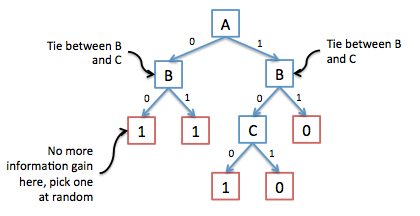
\includegraphics[width=130mm]{tree.jpg}
					\end{center}
				\end{figure}

			\item We would get the same error if we split on whether or not B and C have the same attribute. This shows that ID3 cannot combine properties of more than one attribute when deciding how to split.
				\begin{figure}[H]
					\begin{center}
					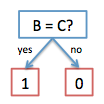
\includegraphics[width=35mm]{tree2.jpg}
					\end{center}
				\end{figure}
		\end{enumerate}
	\item
		\begin{enumerate}
			\item The average ten-fold cross-validation score for the non-noisy data is 0.87 while the score for noise data is 0.78.
			\item 
				\begin{enumerate}
					\item Graph for comparing cross-validation performance over different validation set sizes [1,80]\\
						\begin{figure}[H]
							\begin{center}
							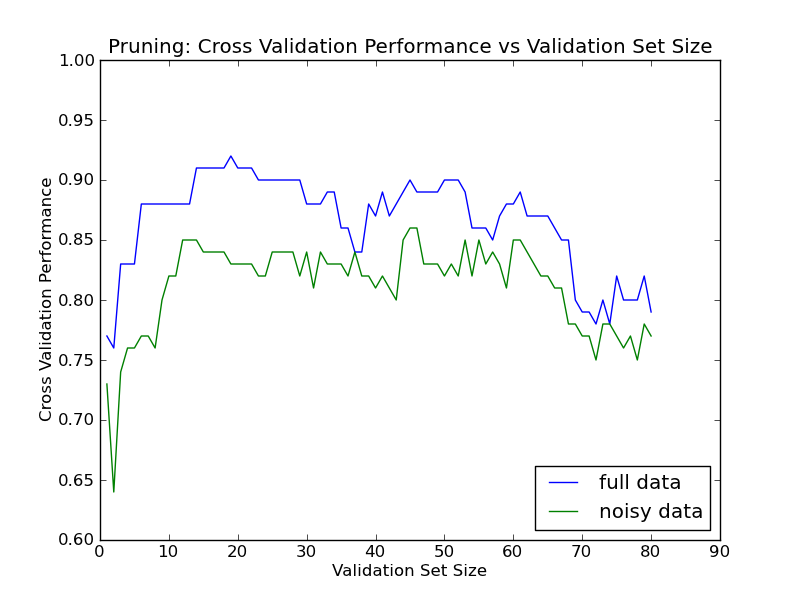
\includegraphics[width=130mm]{2bi.png}
							\end{center}
						\end{figure}
					\item The cross-validation performance was lower for very large or very small validation sets with the performance best at a validation size of around 20 for the full dataset and around 12 for the noisy dataset. The general trend of performance is that it increases from the extreme sizes towards the best performing validation set size ($\sim$19)
					\item As shown in the graph below, for the full dataset, validation set pruning did not improve or slightly to moderately decreased the cross-validation set performance for larger ($>$ 40) or smaller ($<$10 ) validation set sizes. For the sizes of around 10 to 40, validation set pruning did improve the cross-validation set performance though the improvement is slight. For the noisy dataset, validation set pruning made higher improvements on the cross-validation performance than for the full dataset. This made sense since spurious irrelevant patterns would be more common if there were noise in the data. However, the improvement is still small\\
					\begin{figure}[H]
							\begin{center}
							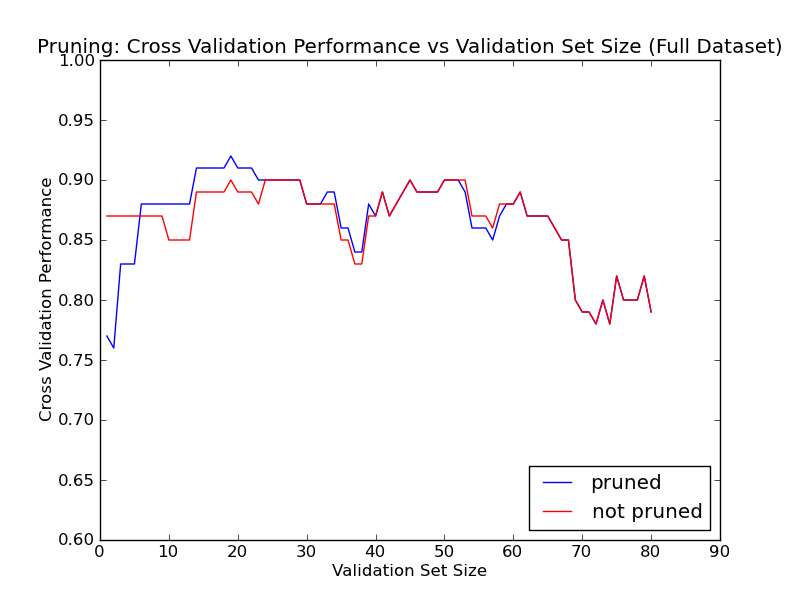
\includegraphics[width=130mm]{2biii1.png}
							\end{center}
						\end{figure}
						\begin{figure}[H]
							\begin{center}
							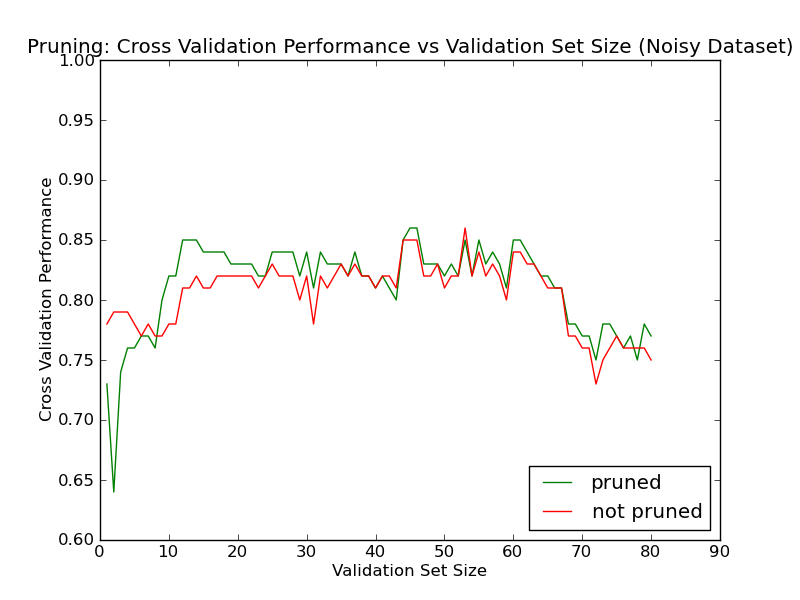
\includegraphics[width=130mm]{2biii2.png}
							\end{center}
						\end{figure}
					\item Overfitting is an issue for these data, though not a big issue. Overfitting happens when we have a decision tree that is too specific for the training data and fails to generalize to when being tested. Pruning is a technique to prevent overfitting by pruning away the latter branches that are usually more due to spurious patterns than true patterns. While pruning does improve cross-validation performance in the effective ranges ($\sim$10-40), indicating that there is some overfitting, but not too much.
				\end{enumerate}
		\end{enumerate}

	\item
		\begin{enumerate}
			\item We are defining our information gain criterion to be the mutual information between an attribute and the label. However, we will modify all the calculated specific conditional entropies according to the weights of the examples. So instead of:
				\begin{center}
				$H(X|y) = \Sigma_x p(x|y) log_2 \frac{1}{p(x|y}$
				\end{center}
				We will be replacing the probability distribution $p$ with a weighted distribution based on the weights of the data. This way, data that is "more important" (the ones that tend to be predicted incorrectly) will be weighted more when the algorithm is trying to decide what attribute to split on. Attributes that split the more important data correctly will be favored over those that do not. For the example given where the label of the first example is $y_1 = 1$, etc, the weighted entropy of the set is 
				\begin{center}
				$0.5*log_{2}2 + 0.5*log_{2}2 = 1$.
				\end{center}
			\item
				\begin{enumerate}
					\item 
						Table of how the depth of the tree affects boosting\\\\
    							\begin{tabular}{|c|c|c|}
        							\hline
        							~            & 10 rounds & 20 rounds \\ \hline
        							maxDepth = 1 & 0.93      & 0.92      \\ 
        							maxDepth = 2 & 0.86      & 0.86      \\
        						\hline
    							\end{tabular}
						\\\\A larger maximum depth actually hurts the cross-validated test performance because when the individual trees are more complex, they are more susceptible to overfitting. This introduces trees with splits that are based more on noise than signal.
					\item 
						Boosting performs consistently worse on noisy data compared to non-noisy data no matter how many rounds (from 1 to 30) are performed. This is because the algorithm gives highers weights to data points that are predicted incorrectly. Therefore, if there are inconsistencies within the data, the algorithm will focus on the inconsistent data more than the rest of the data.
						\begin{figure}[H]
						\begin{center}
						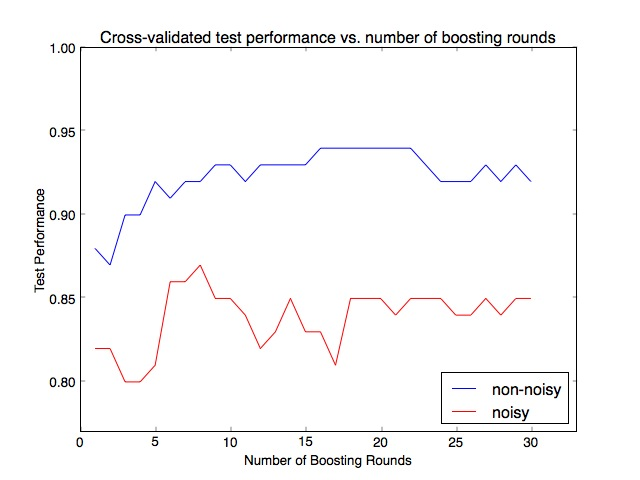
\includegraphics[width=110mm]{figure.jpg}
						\end{center}
						\end{figure}
						
					\item The average performance for boosting reaches a maximum average accuracy of about 0.94 after 10 rounds of boosting as a opposed to a maximum average accuracy of about 0.91 for pruning with a validation set size of 23. Both of these are an improvement over ID3 without pruning, which has a maximum average accuracy of about 0.87. So on this particular non-noisy dataset, pruning is a moderate improvement over un-pruned ID3 and boosting is a moderate improvement over pruned trees.
					\item The algorithm improves with more rounds of boosting both on the training and on the test data. The performance on the test data continues to improve a bit after the performance on the training data plateaus at zero error. This is expected because each individual tree only splits once and thus avoids splitting on an attribute that is not actually important. Because of this, each additional tree does not mold the algorithm to the small nuances of the training data and the algorithm avoids overfitting.
						\begin{figure}[H]
						\begin{center}
						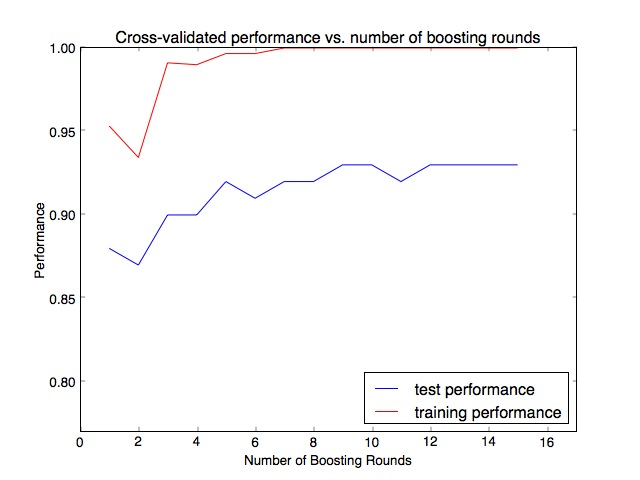
\includegraphics[width=110mm]{figure2.jpg}
						\end{center}
						\end{figure}
				\end{enumerate}
		\end{enumerate}
	\item The following tree was made with the full dataset (total 100 instances) where 71 instances of the data was used for training, 19 instances used for validation-set pruning, and the final decision tree was tested on 10 instances. The model had a score of 1.0 when against the testing set\\
	\begin{figure}[H]
	\begin{center}
	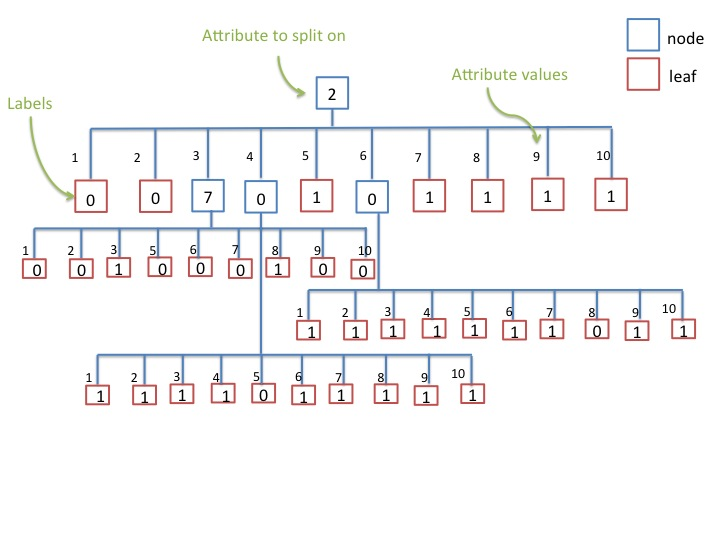
\includegraphics[width=110mm]{4.jpg}
	\end{center}
	\end{figure}
From this tree, we can see that uniformity of cell shape (attribute 2) is the most important attribute in classifying benign vs malignant tumors. In addition, normal nucleoli (attribute 7) and clumping thickness (attribute 0) are also helpful in distinguishing between benign and malignant tumors.

\end{enumerate}
\end{document}